\documentclass[]{article}
\usepackage[spanish.mexico]{babel}
\usepackage[T1]{fontenc}
\usepackage[utf8]{inputenc}
%\usepackage{lmodern}
\usepackage[a4paper]{geometry}

%DIAGRAMAS
\usepackage{smartdiagram}
\usesmartdiagramlibrary{additions}
%ARBOLES
%\usetikzlibrary{trees}

%Plotting

\usepackage{pgfplots}
\pgfplotsset{width=10cm,compat=1.9} 
%\usepgfplotslibrary{external}
%\tikzexternalize 

%Graficos e imagenes
\usepackage{graphicx}
%\graphicspath{ Imagenes/ }
\usetikzlibrary{arrows}

\usepackage{natbib}
\usepackage{cite}

\usepackage{subcaption}

%Grafico de barras
%\usepackage{pgfplots}
%Arrreglos
\usepackage{array}

\usepackage{tikz}
\usepackage[american voltages, american currents,siunitx]{circuitikz}

\title{Efectos de la radiación sobre seres Vivos}
\author{Daniela García Zavala\\ Pablo Vivar Colina}
%Comentar para obtener fecha de HOYs
\date{Octubre 2019}


\begin{document}
	
%%\usepackage[top=2cm,bottom=2cm,left=1cm,right=1cm]{geometry}


\begin{titlepage}
     \begin{center}
	
\includegraphics[width=0.09\textwidth]{UNAM}\Large Universidad Nacional Autónoma de México
        	
\includegraphics[width=0.09\textwidth]{FI}\\[1cm]
        \Large Facultad de Ingeniería\\[1cm]
       % \Large División de Ciencias Básicas\\[1cm]
         \Large Laboratorio de Fundamentos de Control(6655)\\[1cm]
         %la clave antes era:4314
         \footnotesize Profesor: Salcedo Ubilla María Leonor Ing.\\[1cm]
        \footnotesize Semestre 2019-1\\[1cm]
        
       

        \Large Práctica No. 1\\[1cm]
        
           

\Large Introdcción MATLAB
        
         %Texto a la derecha
          \begin{flushright}
\footnotesize  Grupo 2\\[0.5cm]
\footnotesize Brigada: 4\\[0.5cm]
\footnotesize Rodrigo Adrián Martínez López\\[0.5cm]
\footnotesize Vivar Colina Pablo\\[0.5cm]
 \end{flushright}
    %Texto a la izquierda
          \begin{flushleft}
        \footnotesize Ciudad Universitaria Agosto de 2018.\\
          \end{flushleft}
         
          
        %\vfill
        %\today
   \end{center}
\end{titlepage}
 %agregar portada

\maketitle

\tableofcontents  % Write out the Table of Contents

\listoffigures  % Write out the List of Figures


\section{Biología Elemental}

Los efectos de la radiación en los seres vivos se deben a la excitación o ionización de varias moléculas contenidas en las células que forman un sistema vivo. Por lo tanto resulta apropiado revisar algunos conceptos de la biología celular, especialmente células humanas. Cómo sabemos existen aproximadamente $4 x 10^{13}$ células en un adulto promedio. Estas no son idénticas, en función ni en tamaño, la mayoría de las células son bastante pequeñas, en el orden de 10-3 cm de diámetro; las células nerviosas, por el contrario, pueden tener un metro de largo.\\

En esencia el cuerpo humano contiene dos tipos de células las somáticas las cuales componen órganos, tejidos y demás estructuras corporales, y las germinales cómo el espermatozoide y el óvulo, encargados de la reproducción, por ende contienen el material genético hereditario de cada individuo.\\



%En último análisis, el efecto de la radiación en los seres vivos se debe a la excitación o ionización de varias moléculas contenidas en las células que forman un sistema vivo.\\

%Hay aproximadamente $4 x 10^{13}$ células en una persona adulta promedio. Estas, sin embargo, no son todas idénticas, ni en función ni en tamaño. Células cerebrales obviamente realizar una función diferente a las células del hígado. La mayoría de las células son bastante pequeñas, en el orden de $10^{-3}$ cm de diámetro; las células nerviosas, por el contrario, pueden tener un metro de largo.\\

%Las células se dividen en dos grandes clases: células somáticas y células germinales. Casi todas las células del cuerpo son células somáticas. Estas son las células que componen los órganos, tejidos y otras estructuras corporales. Las células germinales, que también se llaman gametos, funcionan solo en reproducción. Es la unión de gametos de diferentes sexos ese es el punto de partida de un nuevo individuo. Los gametos también llevan el material hereditario de la especie que hace que los niños se parezcan más a sus padres que a sus vecinos, y asegura que las debilidades de la humanidad pasen con pocos cambios de generación a generación.\\

%La investigación moderna ha demostrado que la célula viva es un sistema complejo.  

En la figura \ref{celula} se muestra una célula somática típica del tipo encontrado en animales.\\

\begin{figure}[h!]
	\centering
	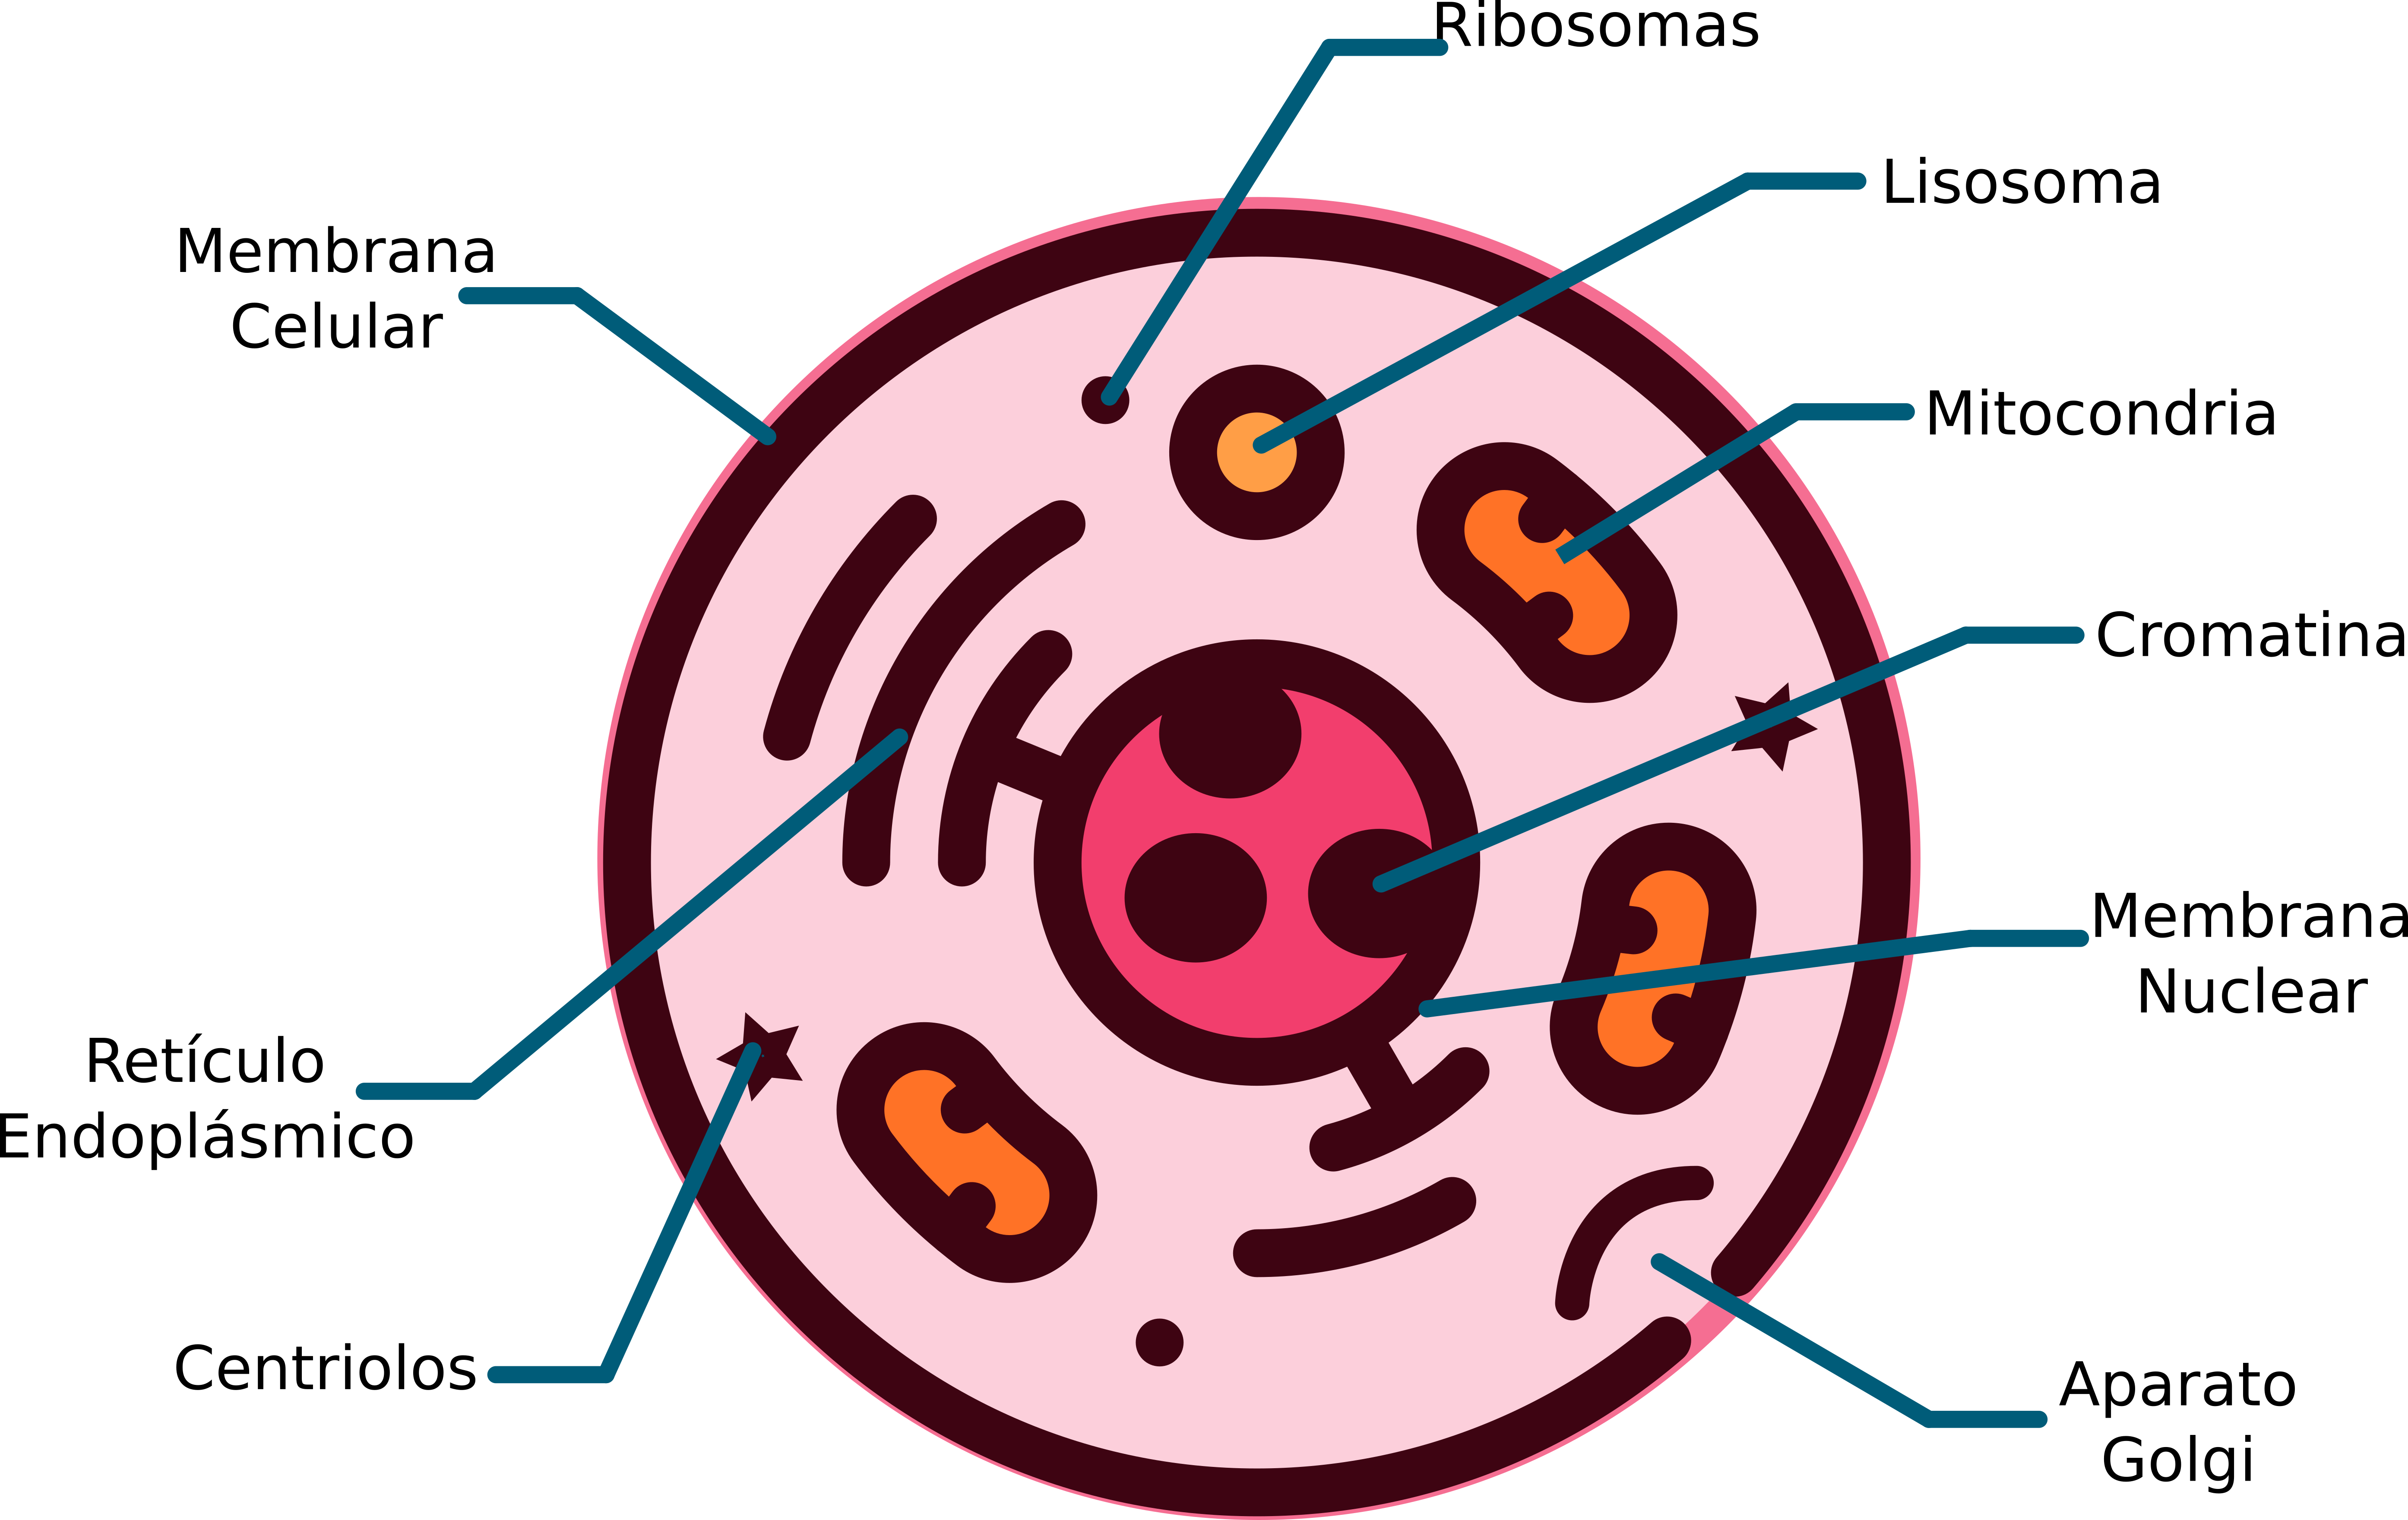
\includegraphics[width=0.6\textwidth]{celula.png}
	\caption{Célula somática tradicional}
		\label{celula}
\end{figure}

%\smartdiagram[constellation diagram]{Tipos de células,
%	, Somáticas, , Germinales}

%\smartdiagram[flow diagram:horizontal]{Edit,
%	\LaTeX, Bib\TeX/ biber, make\-index, \LaTeX}


%\begin{tikzpicture}
%\smartdiagram[bubble diagram:horizontal]{Células,Somáticas,Germinales}{%
%	below of module1/Low Level, below of module3/High level%
%}

\begin{figure}
	\begin{minipage}[t][3.5cm]{\textwidth}
		\begin{center}
			\smartdiagramset{
				%uniform color list=gray!60!black for 3 items,
				back arrow disabled=true,
				additions={
					additional item offset=0.85cm,
					additional item border color=blue,
					%additional arrow color=red,
					%additional arrow tip=stealth,
					%additional arrow line width=1pt,
					%additional arrow style=]-latex’,
				}
			}
		    \smartdiagramadd[bubble diagram:horizontal]{Células,Somáticas,Germinales}{%
				below of module2/Órganos y tejidos, below of module3/Gametos%
			}
		\end{center}
	\end{minipage}
   \caption{}
   \label{tiposCelulas}
\end{figure}


Las células contienen varias estructuras orgánicas llamadas orgánulos, cada una de las cuales realiza funciones específicas para la célula como lo hacen los órganos en el cuerpo como un todo.\\

Estos orgánulos están suspendidos en el citoplasma, una mezcla diluida transparente de agua y diversas moléculas y electrolitos, que comprende la mayor parte de la célula volumen. Otras partes principales de la celda que se muestran en la figura \ref{celula}  son las siguientes:\\

\begin{itemize}
	\item Núcleo. Este es el cuerpo grande, generalmente esférico, que funciona como control central de la célula; Contiene la cromatina.
	 \item Cromatina Este es el material genético de la célula.
	\item Nucleoli (singular, nucleolo). Estos son cuerpos esféricos (puede haber tantos como cuatro ubicados en el núcleo) que son importantes en el metabolismo de ciertos productos químicos.
   \item Retículo endoplásmico. Esta es una red compleja de túbulos aplanados que sirve para transportar materiales dentro de la célula y es también una fuente importante de enzimas metabólicas.
   \item Aparato de Golgi. Las funciones de este orgánulo no se entienden completamente. El Aparato de Golgi aparentemente concentra y modifica ciertas sustancias químicas.
   \item Lisosomas y peroxisomas. Estos orgánulos contienen enzimas para producir diversos productos químicos.
   \item Mitocondrias (singular, mitocondria). Estos objetos (puede haber varios mil en una célula) son responsables del metabolismo de la célula.
   \item Los centriolos. Estos orgánulos ocurren en pares y son esenciales en la división de mitosis o células.
   \item Ribosomas Estos son los centros para la producción de proteínas; Ellos están localizados en el retículo endoplásmico, en la superficie del núcleo y en el citoplasma.
\end{itemize}

El material genético en una célula se llama cromatina solo durante la fase de reposo período de una celda (es decir, cuando la celda no se está dividiendo). En ese momento, aparece como una masa confusa de hebras de moléculas de ácido desoxirribonucleico (ADN), junto con ciertas proteínas nucleares en esta etapa, la cromatina controla la síntesis de las proteínas que le dan a la célula sus características distintivas. Con el inicio de la mitosis, estos hilos se desenredan y se enrollan en un número fijo de paquetes llamados cromosomas, el número de cromosomas varía de una especie a otra; en el hombre, hay 46 cromosomas en cada célula, excepto en las células germinales, que contienen solo la mitad de este número.\\

%NUESTRO 

La división celular ocurre a intervalos de tiempo más o menos fijos durante la vida útil de la célula. El intervalo entre divisiones sucesivas se llama tiempo de ciclo mitótico. El ciclo celular se divide en otros tres intervalos, como se ilustra en la figura  \ref{fig:repCelular}.\\

En la mitosis, cada cromosoma se duplica exactamente, así que cada célula recién formada adquiere un complemento completo de 46 cromosomas. Ya que el ADN cromosómico controla la producción de proteína celular, las dos nuevas células desarrollarse son réplicas de la célula original. Después de la mitosis, los cromosomas se desenrollan y volver a su antiguo estado enredado. Sin embargo, es importante tener en cuenta que, aunque en esta etapa no se pueden distinguir los cromosomas individuales, todavía existen como entidades específicas. La cromatina, en resumen, está compuesta de cromosomas desenrollados, no cromosomas desintegrados.\\

La división celular ocurre a intervalos de tiempo más o menos fijos durante la vida útil de la célula. El intervalo entre divisiones sucesivas se llama tiempo de ciclo mitótico. El ciclo celular se divide en otros tres intervalos, como se ilustra en la figura \ref{mititicCycle} \\

\begin{figure}[h!]
	\centering
	\begin{subfigure}[b]{0.45\textwidth}
		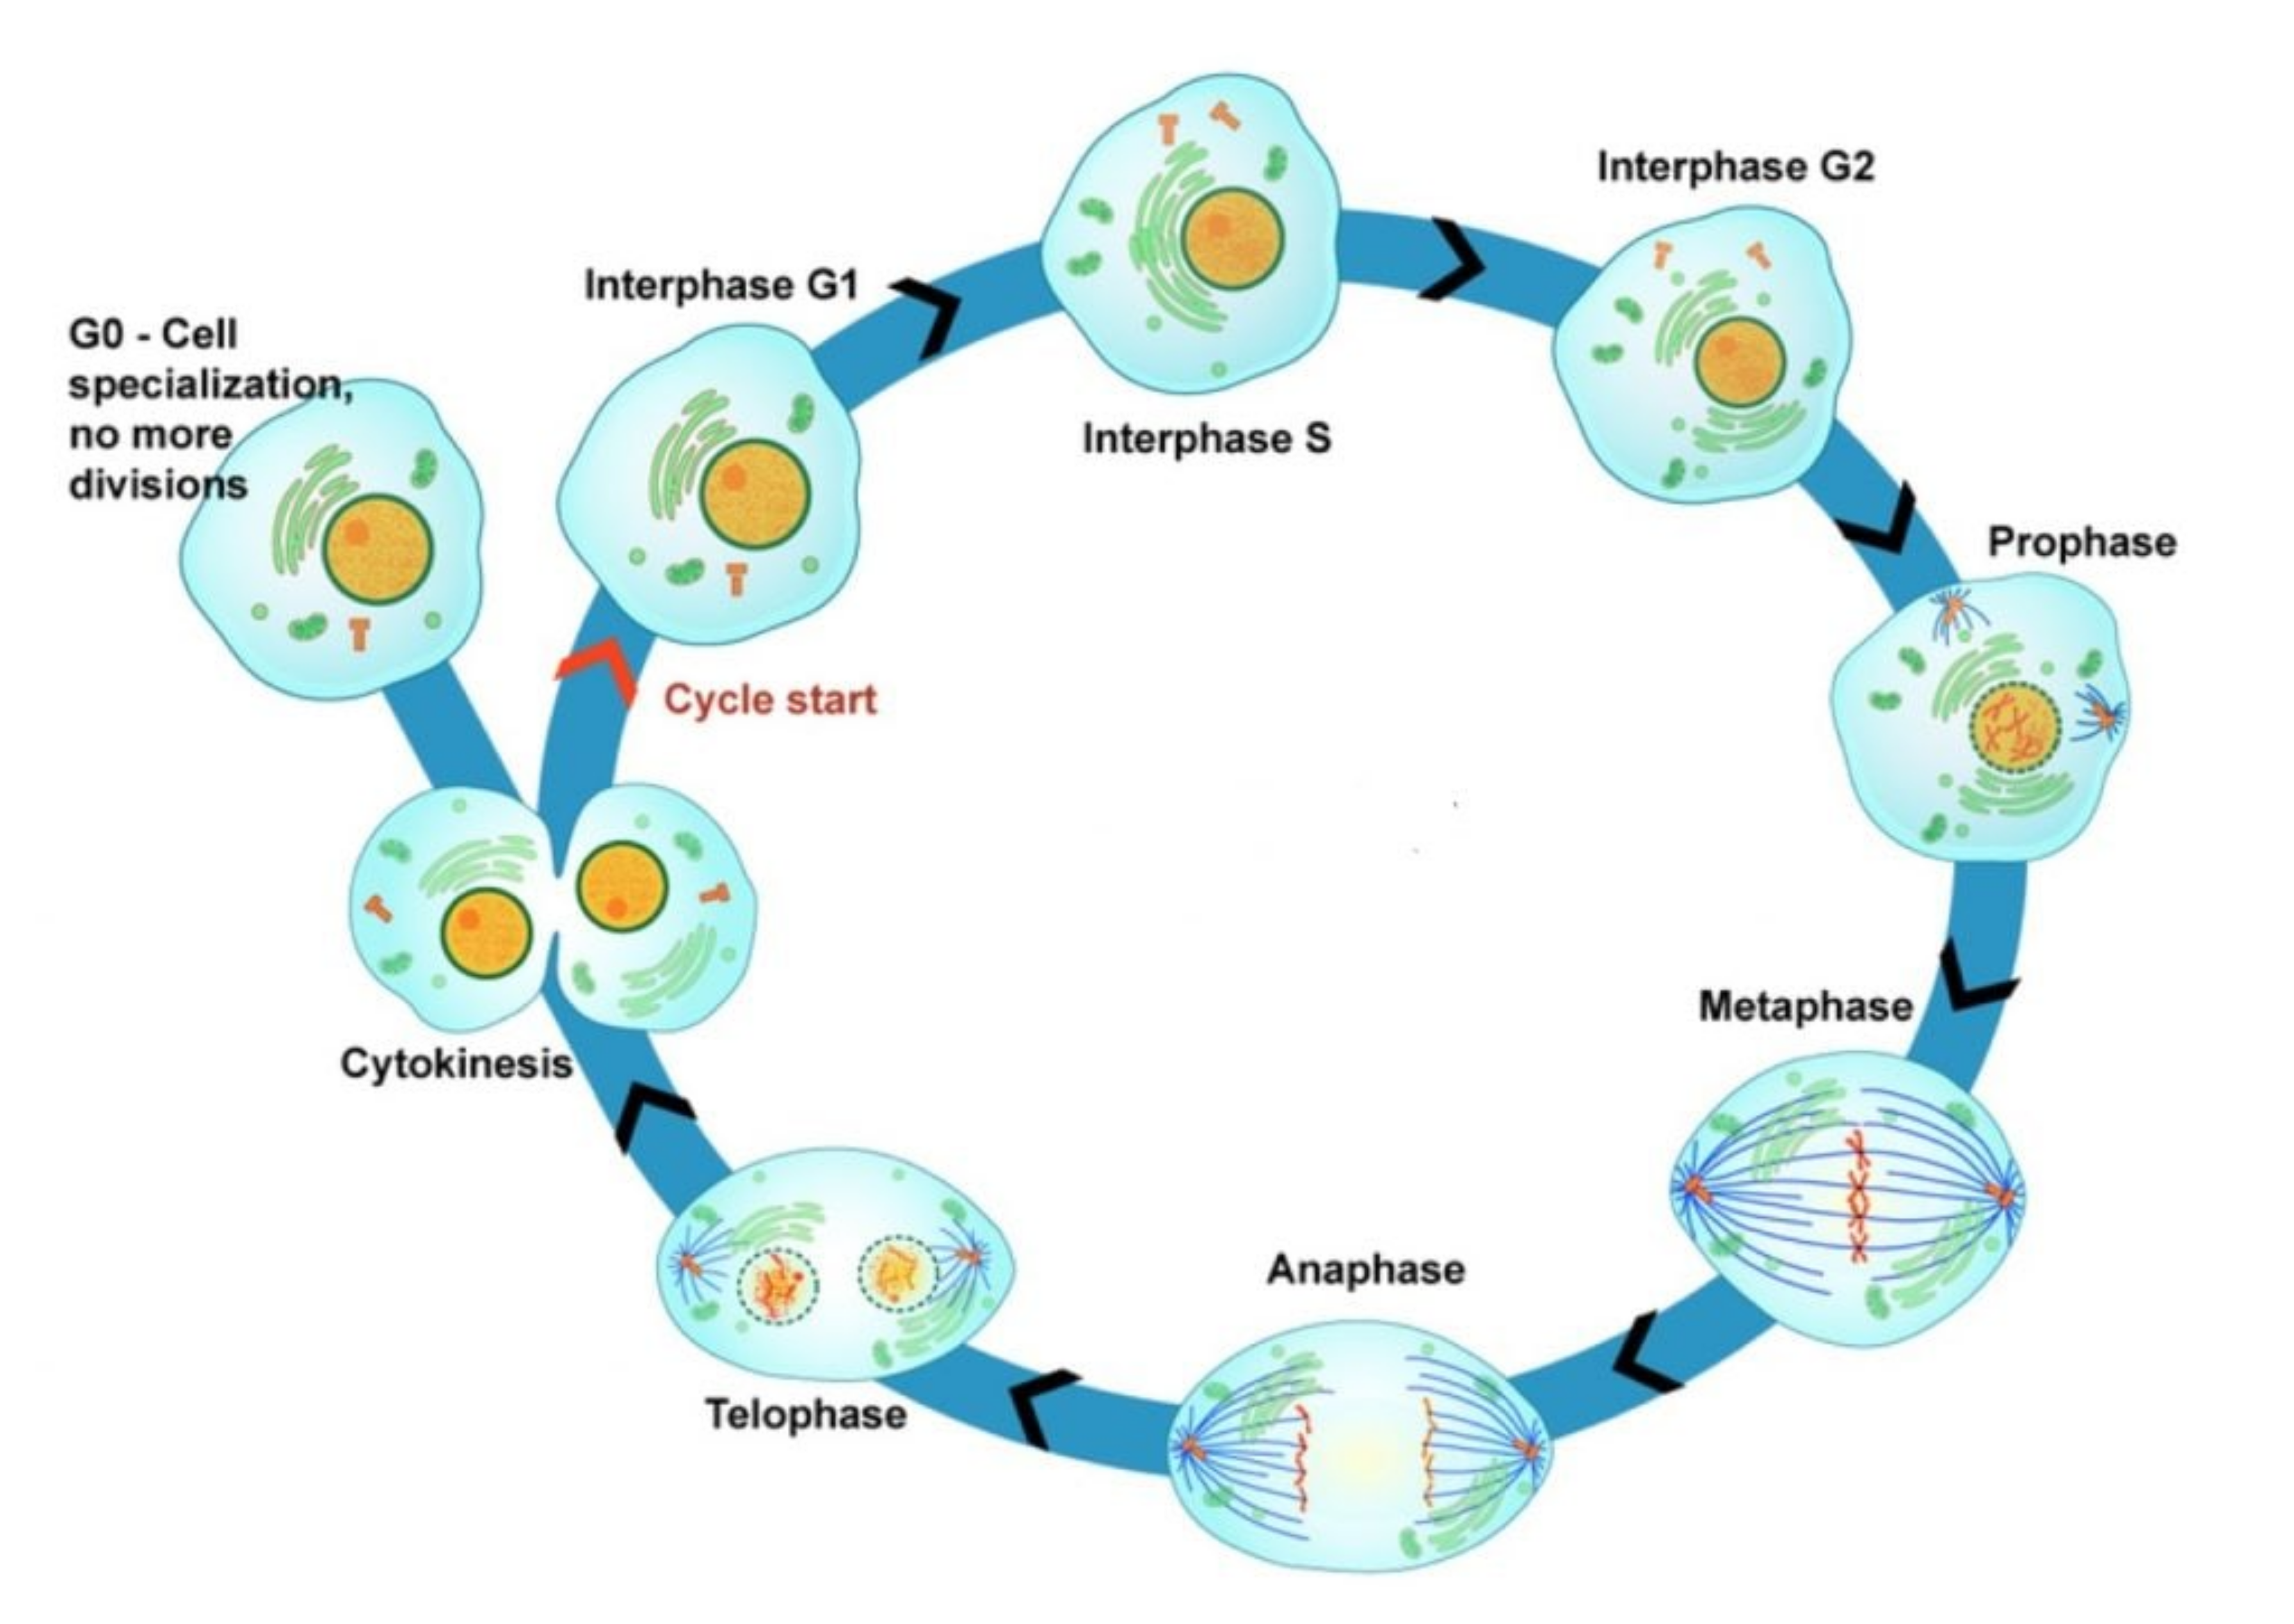
\includegraphics[width=\textwidth]{mitosis.png}
		\caption{Etapas reproducción celular}
		\label{fig:repCelular}
	\end{subfigure}
	~
	\begin{subfigure}[b]{0.3\textwidth}
		\begin{tikzpicture}[]
		    %\draw[] (0,0) arc (0:220:1);
		    \draw[]
		    (0,0) circle (1.75)
		    (0,0) circle (2)
		    (0,0) circle (2.3)
		    ;
		    \draw[rotate={70}](1.75,0)--(2.5,0);
		    \draw[rotate={110}](1.75,0)--(2.5,0);
		    \draw[rotate={230}](1.75,0)--(2.5,0);
		    \draw[rotate={300}](1.75,0)--(2.5,0);
		    %\fill[black] (-0.05,0) -- (0.05,0) -- (0,0.1);
		    
		    %PRIMER PAR DE FLECHAs
		     \fill[black,rotate={70}] (0+2.3,0)--(0.05+2.3,0.1) -- (-0.05+2.3,0.1);
		    \fill[black,rotate={70}] (0+2.3,0)--(0.05+2.3,-0.1) -- (-0.05+2.3,-0.1);
		     
		     %Segundo PAR DE FLECHAs
		     \fill[black,rotate={110}] (0+2.3,0)--(0.05+2.3,0.1) -- (-0.05+2.3,0.1);
		     \fill[black,rotate={110}] (0+2.3,0)--(0.05+2.3,-0.1) -- (-0.05+2.3,-0.1);
		     
		     %TERCER PAR DE FLECHAs
		     \fill[black,rotate={230}] (0+2.3,0)--(0.05+2.3,0.1) -- (-0.05+2.3,0.1);
		     \fill[black,rotate={230}] (0+2.3,0)--(0.05+2.3,-0.1) -- (-0.05+2.3,-0.1);
		     
		     %CUERTO PAR DE FLECHAs
		     \fill[black,rotate={300}] (0+2.3,0)--(0.05+2.3,0.1) -- (-0.05+2.3,0.1);
		     \fill[black,rotate={300}] (0+2.3,0)--(0.05+2.3,-0.1) -- (-0.05+2.3,-0.1);
		     
		    %ARRIBA
		    %\fill[black] (0,0)--(0.05,0.1) -- (-0.05,0.1);
		    %DERECHA
		    %\fill[black] (0,0)--(0.1,-0.05) -- (0.1,0.05);
		    %IZQUIERDA
		    %\fill[black] (0,0)--(-0.1,-0.05) -- (-0.1,0.05);
		    %ABAJO
		    %\fill[black] (0,0)--(0.05,-0.1) -- (-0.05,-0.1);
		    
		    \node[] at(2.6,0){$G_1$};
		    \node[] at(-2.6,0){$G_2$};
		    \node[] at(0,3){$M$};
		    \node[] at(0,2.6){(mitosis)};
		    \node[] at(0,-2.6){S (Síntesis ADN)};
		\end{tikzpicture}
     \caption{Ciclo mitótico de una célula}
     \label{mititicCycle}
   \end{subfigure}
	\caption{Reproducción Celular}
	\label{repCelularGanz}
\end{figure}

En la figura (\ref{mititicCycle}), $M$ es el tiempo durante el cual tiene lugar la mitosis. Durante el intervalo $S$, en la mitad del ciclo, el ADN se sintetiza en el núcleo. Los intervalos $G_1$ y $G_2$ se conocen como brechas en el ciclo. El núcleo celular está relativamente inactivo en estos tiempos. En las células pulmonares y ováricas de los hámsteres recién nacidos, que son comúnmente utilizado en experimentos radiobiológicos, $M = I$ $h$, $S = 6$ $h$, $G_1 = 1$ $h$ y $G_2 = 3$ horas el tiempo total del ciclo es, por lo tanto, 11 horas. Las células de otros animales y tejidos tienen diferentes tiempos de ciclo. En las células madre basales del intestino humano, el mitótico el tiempo de ciclo es de aproximadamente 24 horas. Por otro lado, las células nerviosas y musculares, por ejemplo, están altamente diferenciados; tienen una vida larga y esencialmente nunca se someten mitosis.\\

\begin{figure}[h!]
	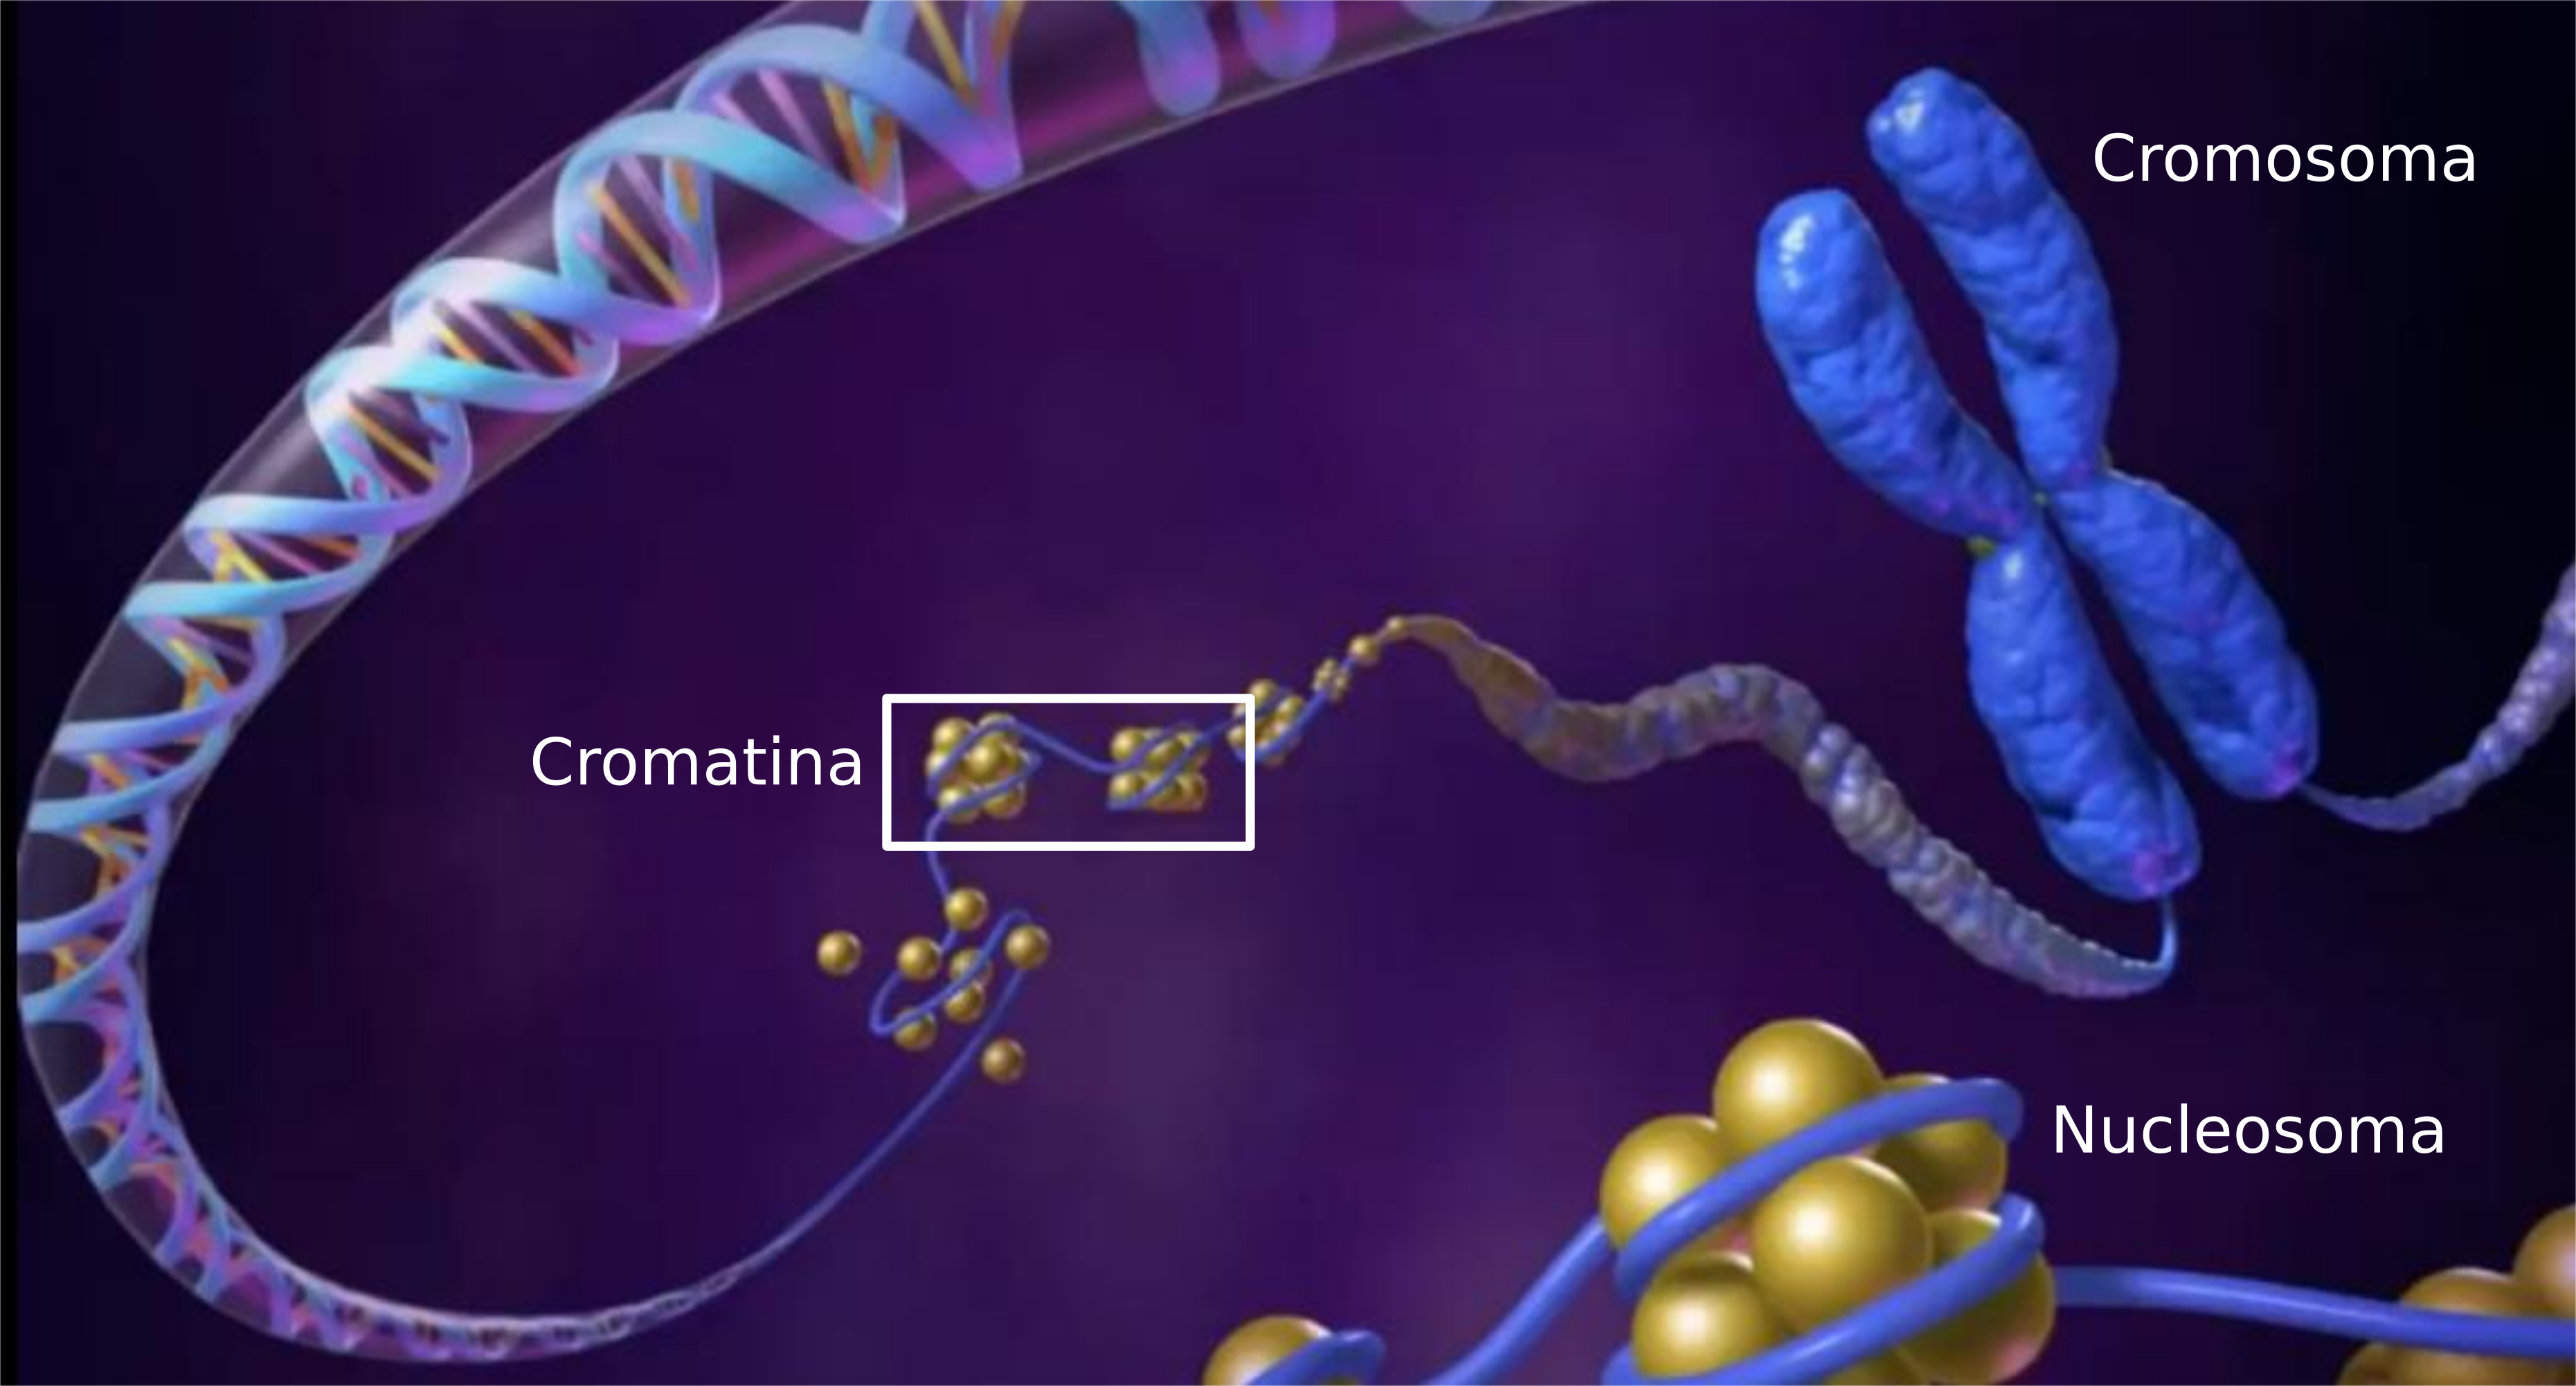
\includegraphics[width=\textwidth]{ADN.png}
	\caption{ADN condensándose en cromosomas}
\end{figure}

%La estructura de las células germinales es muy diferente de la de las células somáticas y No será discutido aquí. En cualquier caso, hay dos variedades de células germinales. Estas se llaman, respectivamente, espermatozoides y huevos u óvulos (singular, óvulo). Los primeros se producen en los testículos del hombre, los segundos en los ovarios de la mujer.\\

Colectivamente, los testículos y los ovarios se llaman gónadas. En reproducción, la unión de un espermatozoide y un óvulo, cada uno con 23 cromosomas, produce un cigoto, el primer paso para originar un nuevo individuo. El cigoto contiene 46 cromosomas. La mitosis del cigoto y su progenie finalmente produce una descendencia de tamaño completo.\\

%Durante muchos años, se pensó que las características hereditarias se derivan de las acciones de genes individuales, que fueron representados como entidades similares a partículas encadenadas a lo largo de los cromosomas. Ahora se sabe que los genes son en realidad segmentos de Moléculas de ADN que proporcionan un tipo de código que controla la síntesis de proteínas.\\

%Sin embargo, el término $gen$ todavía se usa para describir el punto de origen de reconocible características y cambios en los cromosomas que dan como resultados nuevos, heredables, las características se denominan mutaciones genéticas.\\

\section{Los efectos biológicos de la radiación}

Es habitual dividir los efectos biológicos de la radiación en dos clases amplias, dependiendo sobre si los efectos son inherentemente estocásticos o no estocásticos en naturaleza. Los efectos estocásticos son aquellos cuya probabilidad de ocurrencia, en oposición a severidad, se determinan por dosis. El cáncer y las mutaciones genéticas son ejemplos de Efectos estocásticos. Como se discute a continuación, existe una probabilidad definitiva de que el cáncer resultado de una dosis de radiación dada, pero de ninguna manera es seguro que el cáncer resulte de esa dosis, además, la magnitud o gravedad máxima del cáncer no está relacionado con la dosis original; está determinado por eventos y circunstancias que ocurrirá mucho después del evento iniciador. Con procesos estocásticos, no hay razón suponer que hay algún nivel de radiación por debajo del cual no es posible ningún efecto.\\

Presumiblemente, cualquier dosis, por pequeña que sea, es capaz de iniciar un efecto estocástico. Los efectos no estocásticos o deterministas de la radiación son completamente predecibles, y su gravedad es una consecuencia inevitable de una dosis dada. Ejemplos de no estocásticos son los efectos son daños cutáneos no malignos (eritema), la forma de cataratas (opacidad de la lente del ojo), efectos hematológicos (cambios en la composición de la sangre), y así sucesivamente. Tales procesos no estocásticos pueden requerir algún tipo de dosis umbral antes de que se manifiesten, como en el caso de catarata, pero, ya sea que haya un umbral o no, la gravedad de la lesión finalmente aumenta con el nivel de la dosis.\\



\begin{figure}[h!]
	\begin{minipage}[t][3.5cm]{\textwidth}
		\begin{center}
			\smartdiagramset{
				%uniform color list=gray!60!black for 3 items,
				back arrow disabled=true,
				additions={
					additional item offset=0.85cm,
					additional item border color=blue,
					%additional arrow color=red,
					%additional arrow tip=stealth,
					%additional arrow line width=1pt,
					%additional arrow style=]-latex’,
				}
			}
			\smartdiagramadd[bubble diagram:horizontal]{Efectos de la radiación,Estoclásticos,No estoclásticos}{%
				below of module2/Determina por dosis Cáncer Mutaciones, below of module3/Predecibles Efectos hematológicos%
			}
		\end{center}
	\end{minipage}
	\caption{}
	\label{efectosRadiacion}
\end{figure}

\subsection{Mecanismos de los efectos de la radiación.}

Debido a que la célula es un sistema tan complejo, no puede haber un efecto único de radiación,
incluso a nivel celular. Cualquier efecto que ocurra dependerá necesariamente sobre qué orgánulos están involucrados y sobre su importancia para el funcionamiento de la célula. Hay dos mecanismos fundamentales por los cuales la radiación puede afectar un organelo Primero, la radiación puede conducir a la ruptura de moléculas, rompiendo sus enlaces por el efecto ionizante de la radiación, esto se conoce como el efecto directo de radiación. Segundo, la radiación, nuevamente debido a su poder ionizante, puede resultar en producción de nuevos productos químicos, como el oxi altamente reactivo (0) y el hidroxilo (OH) radicales, que interactúan químicamente dentro de la célula. Esto se llama un indirecto Efecto de la radiación. La evidencia experimental reciente sugiere que el efecto indirecto es más importante en gran medida en producir efectos biológicos. En cualquier caso, es importante reconocer que ambos procesos son fundamentalmente químicos en la naturaleza: una falla en la molécula es necesariamente otras dos moléculas. Los efectos biológicos de la radiación, por lo tanto, no son esencialmente diferentes de los efectos biológicos de varios productos químicos. La radiación es simplemente un medio diferente y aparentemente extraño para producir los productos químicos en cuestión.\\

El resultado final de estas transformaciones químicas en una célula depende de qué moléculas celulares se ven afectadas. Los detalles de estos procesos no son enteramente entendidos en la actualidad. Sin embargo, hay evidencia abrumadora que, con respecto a los efectos estocásticos y no estocásticos observables, los más sensibles partes de la célula se encuentra dentro del núcleo celular, probablemente con los cromosomas.\\

Otros organelos pueden verse afectados por la radiación, por supuesto. Si uno de los mayores moleculares estructuras en una mitocondria se dañan, por ejemplo, el funcionamiento de este, los orgánulos pueden ser interrumpidos. Sin embargo, debido a que hay muchas mitocondrias en la mayoría células, el mal funcionamiento de una de estas estructuras normalmente no tendría observables efectos sobre el comportamiento general de la célula. Pero los eventos que tienen lugar dentro de los núcleos son cruciales para el bienestar de la célula en su conjunto y pueden transmitirse a la progenie celular en la mitosis.\\

\section{Muerte Celular}

Es posible extraer porciones de tejido de varios órganos animales para extraer células individuales, y hacerlas crecer en colonias celulares sanas y multiplicadoras. Esto es generalmente se hace en recipientes planos y poco profundos llamados placas de Petri, que contienen un adecuado medio cultural. Cuando tales colonias están expuestas a la radiación durante un período corto (es decir, cuando reciben dosis agudas de radiación), una fracción de las células expuestas deja de reproducirse y finalmente se desintegra. En este caso, se dice que las células han sido asesinadas por la radiación; más exactamente, han sufrido de lo que es llamada muerte reproductiva.\\

Cuando la fracción de células supervivientes se representa frente a la dosis de radiación, la supervivencia Se obtienen curvas como las que se muestran en la figura \ref{radiacionLET}. En todos los casos, los sobrevivientes la fracción disminuye con los aumentos en la dosis absorbida, como se esperaría. Sin embargo, como se indica en la figura, hay una marcada diferencia para un determinado absorción de dosis entre las fracciones de supervivencia con radiación LET (Linear Energy Transfer/Transferencia lineal de energía) alta y baja. Con altura LET radiación, la fracción de células supervivientes cae bruscamente (exponencialmente), pero con baja radiación LET, la curva de supervivencia exhibe cierta planitud u $hombro$ en dosis bajas y solo cae abruptamente a dosis altas.\\

\begin{figure}[h!]
	\centering
	\begin{tikzpicture}
	
	 
	%\draw (-2,0) -- (2,0);
	%\filldraw [gray] (0,0) circle (2pt);
	%CURVA BEZIER CON 3 PUNTOS
	\draw [blue,thick](0,9) .. controls (4,7.5) .. (9,1);
	%CURVA ROJA
    \draw[red,thick](0,9)--(3,1);	
	\draw[thick]
	  (0,0)--(10,0)
      (0,0)--(0,10)
      ;
     \draw[thick]
     %marca200
     (1.6,0)--(1.6,0.5)
      %marca400
     (3.4,0)--(3.4,0.5)
      %marca600
     (5,0)--(5,0.5)
     %marca800
     (6.6,0)--(6.6,0.5)
     %marca1000
     (8.4,0)--(8.4,0.5)
     %marca1200
     (10,0)--(10,0.5)
     ;
     \draw[dashed,gray]
      (0,3)--(10,3)
      (0,6)--(10,6)
      (0,9)--(10,9)
      ;
	%\draw (-2,2) .. controls (-1,0) and (1,0) .. (2,2);
	
	\node[] at(1.6,-0.5){200};
	\node[] at(3.4,-0.5){400};
	\node[] at(5,-0.5){600};
	\node[] at(6.6,-0.5){800};
	\node[] at(8.4,-0.5){1000};
	\node[] at(10,-0.5){1200};
	
	\node[] at(5,-1.5){Radiaciones};
	
	\node[] at(-0.5,0){$10^{-3}$};
	\node[] at(-0.5,3){$10^{-2}$};
	\node[] at(-0.5,6){$10^{-1}$};
	\node[] at(-0.5,9){1};
	
		\node[rotate={90}] at(-1.5,4.5){Fracción superviviente};
	\draw[gray] (6,7) rectangle (11,8.5);
	\draw[red,thick](6.5,8)--(7.25,8);
	\draw[blue,thick](6.5,7.5)--(7.25,7.5);
	\node[] at(9,8){Radiación LET Alta};
	\node[] at(9,7.5){Radiación LET Baja};
	

	
	
	\end{tikzpicture}
	\caption{Curvas de supervivencia de células expuestas a dosis agudas de radiación}
	\label{radiacionLET}
\end{figure}

Actualmente no es posible una explicación precisa de las curvas de supervivencia celular. hora. Está claro, por supuesto, que el efecto de la alta radiación LET es mayor que el de baja radiación LET por dosis absorbida, que es otra forma de decir que El RBE es más grande para la radiación LET alta. La existencia del hombro con baja LET radiación a dosis bajas sugiere la existencia de algún tipo de umbral para este tipo de radiación, posiblemente debido a mecanismos de reparación dentro de la célula que son abrumado a altas dosis. Al menos está claro que la relación dosis-efecto está lejos menos directo a dosis bajas que a dosis altas. Estas características generales de alta y La baja radiación LET se encuentra en prácticamente todos los datos relacionados con los efectos biológicos de radiación.\\

Se recordará de la sección anterior que las células tienen un ciclo mitótico natural. Durante el cual ocurren diversas actividades en momentos específicos. Usando un número de Técnicas sofisticadas, los biólogos pueden producir colonias de células cuyos ciclos son todo en fase. Es decir, todas las células sufren mitosis al mismo tiempo, producción de ADN. al mismo tiempo, y así sucesivamente. Se dice que tales células o colonias son sincrónicas.\\

Cuando las células sincrónicas se irradian en varios puntos de sus ciclos mitóticos, se encuentra que el efecto de la radiación, tanto de baja LET como de baja LET, es algo más pronunciado justo antes o durante la mitosis. Células irradiadas en otros puntos del ciclo tiende a sobrevivir al efecto de la exposición a la radiación hasta el inicio de la mitosis, cuando no se reproducen y mueren una muerte reproductiva.\\

Los experimentos con células sincrónicas explican el fenómeno de radiosensibilidad, que se observa para los efectos estocásticos y no estocásticos de radiación en organismos enteros, incluido el hombre. Por lo tanto, ciertos tejidos, a saber, aquellos cuyas células se reproducen con mayor frecuencia, normalmente son las más sensibles a la radiación.\\

Estas células a menudo mueren cuando intentan la mitosis; si sobreviven a la mitosis, pueden sensibilizarse para la posterior inducción de cáncer. Dichos tejidos radiosensibles incluyen la médula roja, que produce continuamente nuevas células sanguíneas, y el tejido debajo del revestimiento del tracto gastrointestinal que contiene las células madre que continuamente reemplazar el revestimiento del tracto. Por el contrario, cuanto más estático es el tejido muscular y los huesos, por ejemplo, son mucho más inmunes a los efectos de la radiación.\\

Las observaciones anteriores, especialmente con respecto a los tejidos radiosensibles, relacionarse solo con el cuerpo después del nacimiento. Antes del nacimiento, o en el útero, todos los tejidos fetales están experimentando un rápido desarrollo y, por esta razón, son particularmente sensibles a la radiación Este es especialmente el caso durante el período embrionario, desde fertilización hasta aproximadamente la octava semana.\\

La muerte celular, que es claramente un proceso no estocástico, explica la clínica efectos (es decir, los efectos médicos graves) que se observan después de la exposición aguda de individuos a la radiación. Estos efectos, descritos en detalle en la siguiente sección, dependerá de cuántas células se maten y de la función normal o el propósito de Células.\\

Considere, por ejemplo, la irradiación de los intestinos. El revestimiento del intestino se renueva continuamente por la multiplicación de células justo debajo del revestimiento superficie. Cuando el intestino está expuesto a los rayos Y, la tasa de producción de estos las células se ralentizan. Hasta dosis de radiación moderadas, se forman suficientes células nuevas para mantener la pared intestinal, Sin embargo, a dosis altas, la superficie no puede mantenerse, y se desintegra Como consecuencia, varios fluidos corporales ingresan a los intestinos, mientras que los materiales bacterianos y tóxicos del intestino pasan a la sangre corriente. El efecto general sobre el individuo es diarrea, deshidratación, infección y toxemia (envenenamiento de la sangre). Como muestra este ejemplo, los resultados de la participación de todo el cuerpo de eventos a nivel celular.\\

\section{Cáncer}

El cáncer es la segunda causa de muerte en el mundo de hoy.

%DATOS EN MEXICO

%En los Estados, aproximadamente el 38 $\%$ de la población contrae la enfermedad, y 17 $\%$ sucumbe lo. De los 275 millones de personas que vivían en este país en 2000, alrededor de 47 millones de ellos morirán de cáncer si las tasas de mortalidad por cáncer no cambian. Actual Las tasas de mortalidad para varios tipos de cáncer en los Estados Unidos se dan en el cuadro \ref{mortandadCancer}.\\


%REVISAR HOJA
\begin{table}[h!]	
	\centering
	\begin{tabular}{||c|c|c|c|c||}
		\hline
		\textbf{Tipo de Cáncer }      & \textbf{0 a 17} & \textbf{18 a 29} & \textbf{18 a 29} & \textbf{mayores 60} \\ \hline\hline
			Órganos hematopoyéticos                & 2.41 & 2.48 & 3.96 &   \\ 
			Huesos y de los cartílagos auriculares & 0.33 &      &      &     \\ 
			Tejidos mesoteliales y tejidos blandos & 0.17 &      &      &     \\ 
			Testículo u ovario                     &      & 1.35 & 8.52 & 85*    \\ 
			Mama                                   &      &      & 7.61 & 25.23 \\ 
		    Órganos respiratorios e intratorácicos &      &      & 3.65 & 50.39 \\ 
			Órganos digestivos                     &      & 1.15 & 15.68& 152.56     \\ 
			Tejido linfático                       & 0.23 & 0.76 &      & \\ 
			Encéfalo y sistema nervioso central    & 0.71 & 0.57 &      &  \\ \hline 
		%Pecho                        & 14.2               \\ 
		%Leucemia                     & 6.3                \\ 
		%Pulmón(Sistema Respiratorio) & 49.5               \\ 
		%Páncreas                     & 8.4                \\ 
		%Estómago                     & 4.2                \\ 
		%Próstata                     & 25.6               \\ 
		%Tiroides                     & 0.3                \\ 
		%Resto                        & 170.1              \\ \hline
	\end{tabular}
%\caption{Tasas de mortalidad por cáncer en los Estados Unidos en 1992-1996 (Muertes por cada cien mil personas por año)}
\caption{Tasa de mortalidad población por edades 2016 por cada 100 00 habitantes \citep{InstitutoNacionalDeEstadisticayGeografia2018}}
\label{mortandadCancer}
\end{table}

El cáncer no se ve ahora como una sola enfermedad, sino más bien como un centenar enfermedades estrechamente relacionadas, todas caracterizadas por una división celular rápida e incontrolada.\\

Hay mil o más químicos, llamados carcinógenos, que son conocidos por producir cáncer Se cree que más del 90 $\%$ de todos los cánceres humanos son resultado de carcinógenos en el medio ambiente, la mayoría de los cuales se producen naturalmente, no hecho por el hombre. Dado que varios productos químicos pueden producir cáncer, no es sorprendente esa radiación también es capaz de hacerlo, en vista del mecanismo subyacente de efectos radiobiológicos descritos anteriormente.\\

Los cánceres inducidos por radiación no son diferentes de los cánceres que surgen de otras causas, por lo tanto, debe deducirse el alcance del efecto inductor de cáncer de la radiación. del aumento (a menudo pequeño) en la incidencia observada de cáncer en grupos de personas expuestas a la radiación. Esto es especialmente difícil en dosis bajas donde el efecto, si es que existe, puede estar oculto en las fluctuaciones estadísticas.\\

Las causas precisas del cáncer no se conocen a partir de este escrito. Hay, sin embargo, evidencia creciente de que la inducción del cáncer es un proceso de dos etapas. En el primero, o iniciación, etapa, se produce una lesión (es decir, alguna lesión u otro efecto perjudicial) en el ADN en una o varias células. Las células afectadas se transforman así en células potencialmente cancerosas, a punto de sufrir una división incontrolada. Sin embargo, algunas personas aún no identificadas, inmunológicas, les impiden hacerlo u otro agente protector. Tales agentes son probablemente características heredadas de cada individuo.\\

Durante la segunda etapa de promoción, el mecanismo de protección falla por alguna razón y permite, las células iniciadas se multiplican sin restricciones. Presumiblemente, La etapa de promoción puede ser provocada por factores tan diversos como las infecciones virales, irritantes químicos, falla del sistema inmunológico o fisiológica cambios en el cuerpo que ocurren naturalmente con el envejecimiento.\\

La teoría del cáncer de dos estados explica el hecho de que hay un período latente de varios años entre el momento de la irradiación y la aparición de muchos tipos de cánceres, durante los cuales la probabilidad de que ocurra un cáncer es esencialmente cero.\\

También explica el hecho de que el cáncer parece darse en familias; es decir, es para en cierta medida un rasgo heredado. Esto también implica, por supuesto, que puede haber segmentos de la población que es especialmente susceptible al cáncer inducido por radiación, una circunstancia que solo recientemente ha sido reconocida. Del mismo modo, probablemente hay segmentos de la población que son especialmente resistentes al cáncer inducido por radiación.\\

Cabe señalar que la célula o las células se desencadenaron en malignidad durante la etapa de promoción generalmente no son las mismas células iniciadas durante la irradiación. Más bien,
son la progenie de las células originales, a menudo eliminadas muchas generaciones. Está despejado, por lo tanto, cualquier carácter iniciador conferido a la célula irradiada debe 
necesariamente ser llevado de generación en generación. De nuevo, esto habla de un cromosoma origen del cáncer.\\

\subsection{Efectos genéticos}

Si la radiación logra alterar una molécula de ADN en un cromosoma, el resultado puede ser una mutación Si esta mutación ocurre en una célula somática de un desarrollo completo individual, no se puede observar ningún efecto macroscópico a menos que se encuentren muchas células igualmente, involucrado Esto se debe a que el ADN determina la estructura de las proteínas.
fabricado por la célula, y una mutación por lo tanto interfiere con la producción de Las proteínas necesarias para el correcto funcionamiento celular.\\

Como resultado, las mutaciones son generalmente dañino para las células y la progenie de una célula mutante, si no la célula madre
en sí, simplemente se extingue. Si la mutación ocurre en una célula germinal, la célula afectada es
generalmente incapaz de ser fertilizado. Sin embargo, si el gameto mutante es exitoso fertilizado y el cigoto se convierte en una descendencia viva, luego se lleva la mutación en la progenie. Por esta razón, la exposición a la radiación de las gónadas es especial. preocupación, al menos a través de la edad reproductiva.\\

Las mutaciones ocurren espontáneamente en la población humana de causas de origen desconocido, De hecho, aproximadamente 10 $\%$ de todos los recién nacidos sufren directamente de un trastorno o mal funcionamiento de origen genético o portar tales defectos, que se expresan más tarde en la vida o en su progenie. Tales defectos pueden ser tan obvios como el albinismo (congénita deficiencia en pigmento de la piel) y síndrome de Down (características mongoloides y retraso mental asociado causado por la presencia de un cromosoma adicional), o tan leves que solo pueden detectarse mediante pruebas de laboratorio. Inducido por la radiación Los defectos genéticos no son diferentes de los normales a la especie. El efecto de la radiación aumenta la tasa de mutación natural.\\

\section{Efecto de la radiación en los humanos}

Se ha realizado un esfuerzo considerable a lo largo de los años para determinar los efectos de la radiación en el cuerpo humano dado que no es posible realizar experimentos de radiación en las personas, el conocimiento actual de los efectos de la radiación se basa en datos de radiación accidentes y sobreexposición; en epidemiológica estudios de enfermedades inducidas por la radiación, como leucemia y cáncer de pulmón; sobre los estudios de las víctimas y sobrevivientes de los bombardeos atómicos de la Segunda Guerra Mundial en Japón; y en numerosos experimentos con animales de laboratorio. La situación actual de estos estudios se puede resumir de la siguiente manera:\\

\begin{enumerate}
	\item Existe información bien documentada sobre los efectos de grandes, agudos (a corto plazo)	dosis de radiación, superiores a 1 0 a 20 rems.
	\item Debido a que los efectos son tan raros, si es que existen, solo hay datos limitados
	mostrando efectos positivos de:	
	\begin{enumerate}
		\item Dosis agudas de hasta 1 0 o 20 rems y no repetidas;
		\item Dosis agudas de algunos rems y repetidas ocasionalmente; y
		\item Dosis crónicas (que continúan durante mucho tiempo) del orden de mili rems por día.
	\end{enumerate}	
\end{enumerate}

%%NO REVISADO A PARTIR DE AQUI%%%%%
Aquí solo se considerarán las categorías (1) y (2-a), ya que son las más importantes para los ingenieros nucleares. Se pueden recibir dosis agudas grandes accidentalmente en una instalación nuclear, mientras que las dosis bajas en la segunda categoría pueden ser la regla en dichas instalaciones.\\

\subsection{Grandes dosis agudas: efectos tempranos}

Al analizar los efectos de las dosis agudas, es habitual distinguir entre los efectos tempranos, que son evidentes dentro de los 60 días de la exposición, y los efectos tardíos, que se hacen evidentes después de 60 días. Los primeros efectos son generalmente de naturaleza no estocástica; Los efectos tardíos surgen de los procesos estocásticos y no estocásticos. El cuadro \ref{cuad:probaPrimEF} muestra los efectos clínicos iniciales tempranos observados después de dosis agudas de todo el cuerpo hasta el orden de 1 000 rems.\\

\begin{table}[h!]
	\centering
	\begin{tabular}{||m{3cm}|m{30em}||}
		 \hline
		\multicolumn{2}{|c|}{Probables primeros efectos de la radiación aguda de el cuerpodosis*t} \\
		\hline	\hline
		Dosis aguda(rems)                                                            & Probable efecto observado                                                                                                                                                                                                                                                                                                                                                                                                                                           \\ \hline
		5 a 75                                                                       & Aberraciones cromosómicas y depresión temporal de los niveles de glóbulos blancos en algunos individuos. No hay otros efectos observables.                                                                                                                                                                                                                                                                                                                          \\ \hline
		75 a 200                                                                     & Vómitos en 5 a 50\% de las personas expuestas en pocas horas, con fatiga y pérdida de apetito, cambios moderados de sangre. Recuperación en pocas semanas para la mayoría de los síntomas.                                                                                                                                                                                                                                                                          \\ \hline
		200 a 600                                                                    & Para dosis de 300 rems o más, todas las personas expuestas exhibirán vómitos dentro de las 2 horas. Cambios sanguíneos severos, con hemorragia y mayor susceptibilidad a la infección, particularmente a dosis más altas. Pérdida de cabello después de 2 semanas para dosis de más de 300 rems. Recuperación de 1 mes a un año para la mayoría de las personas en el extremo inferior del rango de dosis; sólo el 20\% sobrevive en el extremo superior del rango. \\ \hline
		600 a 1, 000                                                                 & Vómitos en 1 hora. Cambios sanguíneos severos, hemorragia, infección y pérdida de cabello. Del 80\% al 1 00\% de las personas expuestas sucumbirán en 2 meses; los que sobrevivan serán convalecientes durante un largo período.                                                                                                                                                                                                                                    \\ \hline
	\end{tabular}
\caption{Probales primeros efectos}
\label{cuad:probaPrimEF}
\end{table}

\subsection{Grandes dosis agudas: efectos tardíos}

Se observará que no se aprecian efectos nocivos graves para dosis de menos de aproximadamente 75 rems. A dosis mayores de 75 rems, se dice que el individuo expuesto sufre de síndrome de radiación aguda.
% o ARS, como se conoce en los círculos médicos.
 Todos los síntomas enumerados en el cuadro \ref{cuad:probaPrimEF} son el resultado de daño simultáneo a varios órganos del cuerpo como resultado, en el tiempo, de lesiones a células individuales como se discutió en la sección anterior.\\

%La incidencia de muerte dada en la Tabla 9.4 es para individuos que no han recibido tratamiento. En este caso, las muertes comienzan a observarse con dosis agudas
%de aproximadamente 200 rems. 

Las personas que reciben tratamiento médico tienen una probabilidad algo mayor de supervivencia; las muertes en este grupo comienzan a ocurrir a aproximadamente 500 rems. La dosis aguda de todo el cuerpo que conduce, sin terapia, a la muerte del 50 $\%$ de un grupo expuesto dentro de los T días de exposición se denomina dosis LDso Por ejemplo, una dosis LDso / 60 matará la mitad de Una población expuesta en 60 días.\\

El LDso / 60 para el hombre no se conoce con precisión, pero se cree que es de aproximadamente 340 rems. Para la mayoría de los mamíferos tiene el mismo valor. Las bacterias y los insectos adultos, por el contrario, tienen un LDso / 60 del orden de 1 0,000 rads.\\

En el rango de dosis de aproximadamente 1 00 a 1 000 rems, los efectos más importantes son los asociados con la sangre, o más adecuadamente, los órganos formadores de sangre, especialmente la médula ósea roja. Se dice que el paciente en este caso exhibe síndrome hematopoyético.\\

La sangre humana consta de tres elementos formados: (1) glóbulos rojos o eritrocitos, (2) glóbulos blancos o leucocitos y (3) plaquetas, todas las cuales están suspendidas en un líquido llamado plasma. Los glóbulos rojos transportan oxígeno, que es necesario para la vida, a través del cuerpo. Las células blancas consisten en varios tipos diferentes de células, las más pobladas son los neutrófilos nucleares polimorfo (50$\%$ -75$\%$) y los linfocitos (20$\%$ -40$\%$). Entre otras funciones que realizan, los glóbulos blancos actúan para repeler o reducir la infección en el cuerpo. Las plaquetas juegan un papel esencial en la coagulación de la sangre.\\

%El rango normal de concentraciones de los elementos de sangre formados (es decir, el conteo sanguíneo normal) se da en la Tabla 9.5. Después de la irradiación aguda de todo el cuerpo, el recuento sanguíneo cambia; la extensión depende de qué tan grande se recibió una dosis. La figura 9.4 muestra un historial típico de recuento sanguíneo después de una dosis aguda de 300 rems.
%Debido a la caída en el número de leucocitos, disminuye la resistencia del individuo expuesto a la infección. Al mismo tiempo, la caída en el recuento de plaquetas previene la coagulación normal de la sangre, lo que, en casos graves, puede provocar hemorragia o sangrado profuso.\\

Cabe señalar que, con la excepción de los linfocitos, que son inusualmente sensibles a la radiación, los otros elementos formados de la sangre son bastante resistente a la radiación. Los cambios del tipo que se muestra en la figura se deben, por lo tanto, a la destrucción de las células madre formadoras de sangre en la médula ósea, pero a la destrucción de las células sanguíneas. El tratamiento para un paciente con síndrome hematopoyético incluye aislamiento en un ambiente estéril, la administraciónde antibióticos y trasplantes de médula ósea.\\

Una dosis aguda de todo el cuerpo de aproximadamente 1, 000 y 5,000 rem conduce a lo que se conoce como síndrome gastrointestinal. En este caso, el efecto dominante y la causa final de muerte es la falla de la pared intestinal debido al agotamiento de sus células madre como se describe en la sección anterior.
El paciente permanece en condiciones satisfactorias durante unos días mientras las células de la pared existentes continúan funcionando, pero a medida que se desprenden, el paciente sucumbe a la infección. El individuo expuesto generalmente muere en dos semanas. 10 Las personas que reciben dosis superiores a 5,000 rems mueren a las pocas horas de la exposición. La causa de la muerte no está del todo clara, pero probablemente implica la rápida acumulación de líquido en el cerebro. Estos síntomas se conocen como síndrome del sistema nervioso central.\\

La discusión anterior se refiere a la irradiación de todo el cuerpo. Si solo una parte del cuerpo está expuesta, los efectos tempranos resultantes dependen de qué parte se irradia, aunque en general se puede decir que la lesión acompañante es siempre menos grave, porque hay menos órganos y sistemas que interactúan. Sin embargo, la exposición puede provocar efectos tardíos graves del tipo que se describirá en breve.\\

Por ejemplo, una mano que recibe una dosis absorbida de 200 a 300 rayos de rayos X exhibirá solo eritema similar a una quemadura solar leve. Las quemaduras más graves, comparables a quemaduras o quemaduras químicas, ocurren con dosis de miles de rads. Aunque en ambos casos la región afectada sanará, se vuelve predispuesta al desarrollo posterior de cáncer de piel.
Grandes dosis agudas: efectos tardíos
Existen datos considerables que muestran los efectos tardíos de la radiación en personas que reciben una gran dosis aguda de todo el cuerpo al menos una vez en la vida. El espacio solo permite un breve resumen de cada efecto.
Cáncer Después de una dosis de radiación aguda, generalmente hay un período cuando
No hay un aumento aparente en la probabilidad de contraer cáncer. La duración del período latente depende de la edad a la que se produce la irradiación y el sitio final de la neoplasia maligna. El período latente es seguido por un intervalo, llamado meseta, donde el riesgo de cáncer es aproximadamente constante. Aquí, el término riesgo se define cuantitativamente como el número de casos de cáncer que se esperan por año después\\

%irradiación por millón de dosis hombre-dosis. Más allá del período de meseta, el riesgo de cáncer cae esencialmente a cero. Se representa un modelo simplificado de riesgo de cáncer i􀚚 Fig. 9.5. La Tabla 9.6 enumera las duraciones del período latente y la meseta para varios tejidos y proporciona los valores de riesgo correspondientes (coeficientes de riesgo).
%Es necesaria una explicación adicional con respecto a los coeficientes de riesgo en la Tabla 9.6.
%Los datos sobre la exposición humana a dosis de radiación aguda superiores a 1 00 rem indican que la incidencia excesiva de cáncer, corregida por los efectos tempranos de la muerte celular, aumenta aproximadamente linealmente con las dosis de radiación baja y alta de LET. Por lo tanto, una gráfica del exceso de incidencia de cáncer versus dosis, llamada curva dosis-respuesta, es una línea recta a dosis altas, como se muestra en la figura 9.6. A dosis más bajas, los datos sobre
la exposición humana es mucho menos concluyente, y la relación de la incidencia de cáncer con la dosis se infiere en su mayor parte de experimentos con animales de laboratorio.\\

Hasta hace poco había una ausencia de datos humanos en dosis bajas. Por lo tanto, la práctica tradicional ha sido extrapolar la curva dosis-respuesta linealmente a una dosis cero, como se indica en la figura. Este procedimiento se conoce como la hipótesis lineal. En general, se acepta que dicha extrapolación es adecuada para la radiación LET alta. Para baja radiación LET, hay evidencia considerable que sugiere que un
La extrapolación lineal sobreestima los efectos cancerígenos de las dosis bajas, y que la curva dosis-respuesta real puede estar por debajo de la curva extrapolada, como se muestra en la figura 9.6. Este tema no se ha resuelto a.s de este escrito y es objeto de un debate considerable.
Los valores de riesgo dados en la Tabla 9.6 se basan en la hipótesis lineal. Los cálculos que utilizan estos valores pueden muy bien exagerar los efectos de la exposición a la radiación a dosis bajas. En cualquier caso, la Tabla 9.6 probablemente proporciona un límite superior para estimar las consecuencias de los accidentes por radiación. Los cálculos de este tipo son descrito en la siguiente sección.\\

\subsection{Mutaciones} 

Los efectos genéticos de la exposición a la radiación en el hombre no han sido
demostrado en la actualidad. En lugar de datos humanos, el riesgo genético de radiación para las personas se estima a partir de datos en ratones de laboratorio. Varios hechos importantes surgen de estos datos. Primero, el ratón macho es considerablemente más sensible a los efectos genéticos de la radiación que la hembra. Exposición de ratones machos a dosis altas
las tasas producen muchas más mutaciones por rem que la misma dosis a tasas más bajas; en otras palabras, una dosis dada hace más daño si se administra durante un período más corto.\\

Por lo tanto, el daño al material genético es claramente reparable. Pero los datos también sugieren que las porciones más sensibles a la radio genética del ratón macho son las espermatozoides y sus espermátidas precursoras, que sobreviven como entidades individuales durante solo una pequeña fracción del ciclo reproductivo. Debido a que lo mismo es cierto en el hombre, esto implica que la transmisión del daño genético de las dosis agudas de radiación puede reducirse retrasando la concepción hasta que las nuevas células espermáticas hayan madurado de células en una etapa menos sensible en el momento de la exposición.\\

%La base para las estimaciones cuantitativas de los efectos genéticos de la radiación en la especie humana es complicada y está más allá del alcance de este libro. 
%(El lector debe consultar las referencias al final del capítulo; ver, en particular, los informes de la Academia Nacional de Ciencias.) 

%En cualquier caso, es habitual dividir tales efectos en las siguientes cuatro clases generales, cada una de las cuales da lugar a uno o más defectos humanos clínicamente observables:

%MIO
Los efectos se pueden representar en las siguientes cuatro clases generales clínicamente observables:

\begin{enumerate}
	\item  Trastornos de un solo gen que surgen de una mutación en un punto específico de un cromosoma.
	\item Trastornos multifactoriales debido a mutaciones de puntos múltiples. (El efecto de la radiación
	en producir tales defectos es difícil de evaluar.)
	\item aberraciones cromosómicas causadas por la presencia de demasiado o muy poco
	material genético en las células (síndrome de Down, por ejemplo).
	\item Abortos espontáneos.	
\end{enumerate}


%La Tabla 9.7 resume los datos sobre el aumento de la incidencia de estos efectos genéticos por 1 06 hombre-rem de una población con una distribución de edad similar a la de los Estados Unidos en 1 970. Los datos incluyen el efecto de la transmisión de defectos genéticos a la subsiguiente generaciones. Dicha propagación se extingue después de aproximadamente tres generaciones.

Debe tenerse en cuenta la gran incertidumbre en el efecto sobre los trastornos multifactoriales.\\

%Cataratas La opacidad de las lentes de los ojos que afecta la visión causada por la radiación, o cataratas por radiación, tiene un período de latencia de aproximadamente 10 meses y puede aparecer hasta 35 años después de la exposición. Son un fenómeno umbral y no ocurren con dosis absorbidas por debajo del rango de 200 a 500 rad para baja radiación LET. Donde la población está expuesta a dosis de todo el cuerpo de este orden de magnitud, habría pocos sobrevivientes con cataratas de radiación. El umbral correspondiente para los neutrones de fisión está cerca de 75 a 1 00 rads. Fertilidad Los efectos probables sobre la fertilidad humana, tanto masculina como femenina, de dosis agudas de rayos y en las gónadas se dan en la Tabla 9.8; datos comparables para neutrones no están disponibles.\\

\subsection{Efectos degenerativos} 

Otro efecto a largo plazo de la exposición a la radiación es un aumento en la incidencia de condiciones degenerativas en varios órganos del cuerpo debido a la falla de los tejidos expuestos para regenerarse adecuadamente. Esto conduce a un deterioro permanente, aunque no necesariamente debilitante, de la función del órgano. La ocurrencia
de tales efectos degenerativos es de esperar en vista del daño que pueden causar grandes dosis a los tejidos y órganos.\\

\subsection{Acortamiento de la vida} 

El efecto general de la exposición a la radiación puede verse en su influencia en la vida útil de las personas expuestas. Esto es claramente de esperar, aunque solo sea sobre la base de los otros efectos a largo plazo que acabamos de comentar. Gran parte de la evidencia de acortamiento de la vida proviene de estudios de obituarios de médicos.\\

Se ha encontrado, por ejemplo, que el promedio de vida de los radiólogos que murieron entre 1 935 y 1 944 fue 4,8 años más corto que el de otros especialistas médicos, que no estuvieron expuestos a la radiación, pero que murieron en el mismo período. En la actualidad, generalmente se cree que cualquier reducción de la vida observada como resultado de la exposición a la radiación se debe únicamente a la aparición de tumores malignos inducidos por la radiación.\\

\subsection{Dosis bajas crónicas} 

Como ya se señaló, las dosis de unos pocos milirems por día, que se acumulan hasta unos pocos rems por año, son motivo de gran preocupación en el desarrollo de la energía nuclear.\\

%Este es el nivel de dosis establecido bajo los estándares actuales de protección radiológica, No es sorprendente, por lo tanto, que se haya hecho un esfuerzo enorme a lo largo de los años para determinar qué efectos perjudiciales, si los hay, acompañan a la exposición crónica a bajos niveles de radiación. Hasta la fecha, los resultados no son concluyentes.\\

%Por lo tanto, 
De acuerdo con el Comité sobre los Efectos Biológicos de las Radiaciones Ionizantes de la Academia Nacional de Ciencias de EE. UU., La derivación de estimaciones de riesgo para dosis bajas y tasas de dosis bajas mediante el uso de cualquier tipo de modelo implica suposiciones que aún deben validarse. Los datos epidemiológicos no pueden excluir rigurosamente la existencia de un umbral en el rango de dosis de milisievert. Por lo tanto, no se puede descartar la posibilidad de que no existan riesgos por exposiciones comparables al fondo natural externo.\\

%tasas de dosis, debe reconocerse que el límite inferior del rango de incertidumbre en las estimaciones de riesgo se extiende a cero.\\

En vista de la evidente falta de datos humanos adecuados sobre los efectos de los bajos niveles de radiación, estos efectos son estimados, o postulados, por varios modelos de dosis-respuesta. Por simplicidad y conservadurismo, a menudo se usa la hipótesis lineal. Existe una gran cantidad de evidencia que sugiere fuertemente que el modelo lineal sobreestima las consecuencias de la exposición crónica a bajos niveles de radiación. De hecho, los datos sugieren que dosis en el rango de 1 0-20 cGy (1 0-20 Rad) pueden ser beneficiosas para reducir las posibilidades de cáncer en niños y adultos. Las dosis superiores a 1 0 cGy siguen siendo potencialmente dañinas para los fetos a las 8-1 5 semanas de gestación, según el análisis de los sobrevivientes de las bombas de Hiroshima y Nagasaki.\\

La hipótesis lineal ignora por completo la capacidad de los sistemas biológicos para repararse a sí mismos, incluso a nivel molecular. Por ejemplo, se ha descubierto que si solo se rompe una cadena de una molécula de ADN (que consta de dos cadenas retorcidas en forma de doble hélice), la molécula puede permanecer intacta y la cadena rota cadena reconstituida en su forma original. Dichos mecanismos de reparación pueden funcionar normalmente a bajas tasas de exposición a la radiación, pero pueden verse abrumados a altas tasas de dosis.\\

La teoría de la hormesis de la radiación sugiere que los organismos responden positivamente a bajas dosis de radiación. Las respuestas incluyen la inhibición del cáncer y la reducción del proceso de envejecimiento. Si bien esta teoría aún está bajo investigación, es completamente consistente con los datos observados de las víctimas de la bomba atómica y con muchos de los otros estudios de caso de radiación.\citep{Lamarsh2001}\\

\section{La radiación LET alta y baja induce de manera diferencial la normalidad
	Señales de daño tisular}

\subsection{Propósito}

 La radioterapia que utiliza radiación de alta transferencia de energía lineal (LET) tiene como objetivo eliminar las células tumorales al mismo tiempo que minimiza la dosis (biológicamente efectiva) a los tejidos normales.
para prevenir la toxicidad. Está bien establecido que una alta radiación LET da como resultado una célula más baja.
supervivencia por dosis absorbida que la radiación LET baja. Sin embargo, si varios mecanismos
que participan en el desarrollo de daño tisular normal puede ser regulado de manera diferencial es
no se conoce. Por lo tanto, el objetivo de este estudio era investigar si dos acciones relacionadas con
a la toxicidad tisular normal, la apoptosis inducida por p53 y la expresión del gen profibrótico
PAI-1 (inhibidor del activador del plasminógeno 1), son inducidos diferencialmente por alto y bajo LET
radiación.

\subsection{Métodos y materiales}

Las células fueron irradiadas con iones de carbono LET alto o fotones LET bajo.
Se realizaron ensayos de supervivencia celular, la expresión profibrótica de PAI-1 fue monitoreada por análisis cuantitativos.
la reacción en cadena de la polimerasa, y la apoptosis fue ensayada por la tinción de la anexión V. Activación de p53
por fosforilación en la serina 315 y la serina 37 fue monitoreada por Western blotting. Transfect--
para el ensayo de los plásmidos que expresan p53 mutados en las serinas 315 y 37 se utilizaron para el ensayo del requisito
de estos residuos para la apoptosis y la expresión de PAI-1.

\subsection{Resultados}

 Como era de esperar, la supervivencia celular fue menor y la inducción de la apoptosis fue mayor en alta -LET
células irradiadas. Interesantemente, la inducción del gen PAI-1 profibrótico fue similar con un alto nivel de glucosa y
baja radiación LET. De acuerdo con este hallazgo, la fosforilación de la p53 en la serina 315 implica
en la expresión de PAI-1 fue similar con radiación LET alta y baja, mientras que la fosforilación de
p53 en la serina 37, involucrada en la inducción de apoptosis, fue mucho más alta después de una alta irradiación de LET.

\subsection{Conclusiones}

Nuestros resultados indican que los diversos mecanismos que intervienen en el desarrollo del
El daño tisular normal puede verse afectado diferencialmente por la radiación LET alta y baja. Esto puede
tienen consecuencias para el desarrollo y la manifestación de daño tisular normal.\citep{Niemantsverdriet2012}\\

\section{Estadísticas del daño del cancer en México}

\begin{enumerate}
	\item Durante el lapso de 2011 a 2016, dos de cada 100 000 habitantes de 0 a 17 años
	fallecen anualmente por un tumor en órganos hematopoyéticos (conformado
	entre otros, por la leucemia). Entre los jóvenes de 18 a 29 años, mueren tres de
	cada 100 000 hombres contra dos de cada 100 000 mujeres por esta causa
	\item Tres de cada 10 muertes por cáncer en la población de 30 a 59 años, son
	consecuencia del cáncer en órganos digestivos. Para la población de 60 y más
	años, de 2011 a 2016, cuatro de cada 10 defunciones por cáncer en mujeres se
	deben a tumor en órganos digestivos, contra tres de cada 10 en varones, por la
	misma causa
	\item Respecto al cáncer de mama, en 2016 se observan 16 defunciones por cada
	100 000 mujeres de 20 años y más
\end{enumerate}

El cáncer es la principal causa de muerte a nivel mundial; en 2015 se calcula que provocó 8.8
millones de defunciones, y se identifican cinco tipos de cáncer responsables del mayor número de
fallecimientos: cáncer pulmonar (1,69 millones de muertes), cáncer hepático (788 000 defunciones),
cáncer colorrectal (774 000 muertes), cáncer gástrico (754 000 defunciones) y de mama (571 000
muertes) (Organización Mundial de la Salud [OMS], 2017).\citep{InstitutoNacionalDeEstadisticayGeografia2018}\\

%A pesar de la posibilidad de que dosis bajas resulten en un efecto positivo, el Comité BEIR y las agencias reguladoras en este momento todavía están utilizando la hipótesis lineal y probablemente continuarán haciendo SO. 13 Existe un consenso cada vez mayor de que la hipótesis lineal es demasiado conservadora, y esto puede conducir a la aceptación de una dosis umbral o incluso a la aplicación de radiación por razones preventivas.\\

\bibliographystyle{plain}
\bibliography{Referencias.bib}

\end{document}
